\documentclass[12pt,a4paper]{article}%
\usepackage[utf8]{inputenc}

%%%% pour ne pas compiler les images
\usepackage{graphicx}
%\usepackage[draft]{graphicx}

\usepackage{geometry}
\usepackage{a4wide}
\usepackage{ulem}
\usepackage{amsmath}
\usepackage{amsfonts}
\usepackage{amssymb}
\usepackage[T1]{fontenc}%
\setcounter{MaxMatrixCols}{30}
\usepackage{hyperref}

\providecommand{\U}[1]{\protect\rule{.1in}{.1in}}
%EndMSIPreambleData
\usepackage{color}
\renewcommand{\@}{\textcolor{red}}
\newcommand{\ed}{\textsc{EcoDyco}}

\date{}

\begin{document}

\newgeometry{top=20mm,bottom=20mm}
\begin{titlepage}

	\centering
		{\Huge \textbf{--- \ed ---} \\[0pt]}
		{\Large Economic Simulation in a World of Finite Resources \\[1cm]}
		\Large Author \textbf{DyCo} \\ 
		\large Universit\'e Paris Cit\'e, CNRS, UMR 8236 \\
		 LIED, F-75013 Paris, France
		\vspace{1cm}

		\begin{figure}[h]
			\centering 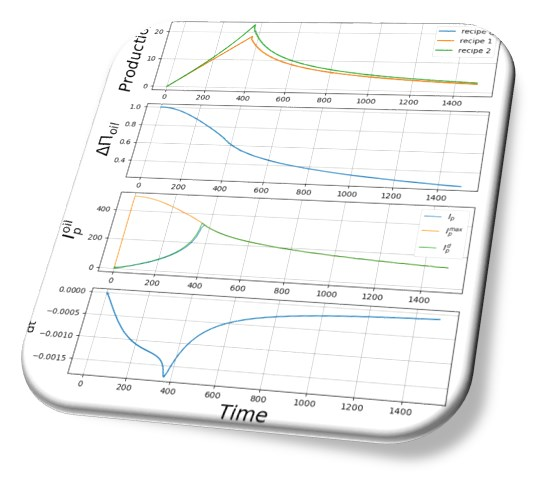
\includegraphics[width=0.9\textwidth]{figures/couverture.jpg}
		\end{figure}
	
		\vspace{1cm}
		{\Huge \textbf{User Manual v1.0} \\[0.5cm]}
		{\Large Sept. 2022 \\[0.5cm]}
		{\large All the material necessary to run the following examples, including this manual, can be found at \url{https://github.com/dyco-uparis/EcoDyco}. 
		}

\end{titlepage}
\restoregeometry

\tableofcontents
\setcounter{page}{1}

\newpage

\section{\ed: Economic Simulation in a World of Finite Resources}

The model \ed\ was designed on the basis of five findings:

\begin{enumerate}
	\item If the physical world is modified by the application of the laws of the economy
	of the economy, the fact remains that its evolution is governed by
	physical laws.
	
	\item The physical world is finite, this is true for all material resources
	resources and for fossil energy resources.
	
	\item In a finite world, the definition of a production function must take into account the state of the resources. Production is contingent on the available resource.
	
	\item The intensity of withdrawal from a resource is a major factor
	on the fate of the resource.
	
	\item If the economy is not strictly describable by thermodynamics,
	thermodynamics can provide it with some useful categories, and in particular the
	In particular, the distinction between \textit{quantity} and \textit{quality},
	themselves linked to the intensive or extensive character of the variables.
\end{enumerate}


\noindent These findings form the basis for the structure and operation of the model \ed.

\begin{enumerate}
	\item The descriptions of the physical and economic spheres of the model
	are disjointed. They communicate through specific variables and parameters. 
	
	\item Each resource is described in its own sheet. The collection of sheets thus obtained is the physical sphere. Each sheet quantifies the usable fraction and the used fraction of the
	Each sheet quantifies the usable fraction and the used fraction of the resource, which we will call waste. The used fraction can only be used again
	used again only after recycling.
	
	\item It is defined a production query function called ``demand'', which
	replaces, for the physical dimension, the production function. The structure and the parameterisation 
	The structure and parameterisation of the production function are fixed by the specific choices
	The structure and parameterisation of the production function are fixed by specific choices made in the economic area of the model.
	
	\item It is defined an intensity of operation of the economy which governs
	the whole of the physical sheets.
	
	\item The quantities of resources are also associated with qualities, which, like the first and second principles, are
	the image of the first and second principles of thermodynamics, define,
	the difference in quality of a resource and its state of transformation, towards a
	transformation, towards a product or towards a waste.
\end{enumerate}


\section{General structure of \ed}

The model is structured in sheets of stock type and flow type,
linked to the economic module. Its overall architecture is shown figure~\ref{fig:globalstructure}.


\begin{figure}[h]
	\centering 
	\includegraphics[width=0.75\textwidth]{figures/Archiglobale.jpg}
	\caption{text}
	\label{fig:globalstructure}
\end{figure}


\subsection{Structure of a Stock sheet}

Stock sheets are intended for most resources, mineral, fossil or not, whose quantity on the planet is finite and of variable dispersion.

\begin{figure}[h]
	\centering
	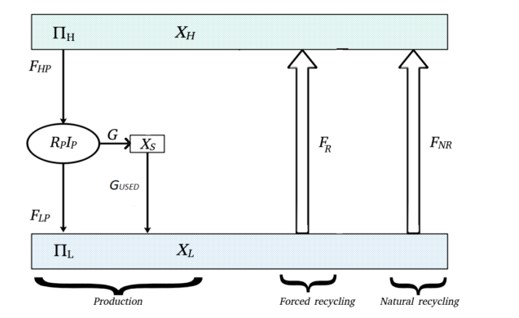
\includegraphics[width=0.75\textwidth]{figures/FeuilleStock.jpg}
	\caption{text}
	\label{fig:StockSheet}
\end{figure}

On a typical stock sheet (figure~\ref{fig:StockSheet}), there is a high zone containing the resource in quantity $X_{H}$ and quality $\Pi_{H}$ and a zone of used resource in quantity $X_{L}$ and quality $\Pi_{L}$. The resource flows of $F_{HP}$ and the waste flows $F_{LP}$ constitute, together with the production flow $G$, the whole of the resource flows in its implementation for production.
The quantity of resource used in excess constitutes a stock $X_{S}$. Recycling can be natural $F_{NR}$, or forced, $F_{R},$ according to specific laws. We call the difference of potentials the quantity $\Delta \Pi=\Pi_{H}-\Pi_{L}$.



\subsubsection{Stock sheet parameters}

A stock sheet is initially defined by the set of limited parameters listed below, values are given as an example.

\begin{itemize}
\item \textit{type : stock}

\item \textit{name : copper}

\item Total quantity --- \textit{total stock : 500000}

\item Initial quantity of high level --- \textit{Xh\_init : 500000}

\item Initial quantity of sink --- \textit{Xl\_init : 0}

\item Production dissipation resistance --- \textit{\ Rp0 : 0.003}

\item Initial capital associated with the
production apparatus --- \textit{\ K0 : 1}

\item Recycling energy ratio (number of energy  unit to recycle 1~unit of the resource) --- \textit{\ recyclingEnergyFlux : 1}

\item Usable as energy (\textit{e.g.} for oil) --- \textit{\ isEnergy : False}

\item Natural recycling rate (r=0~: no recycling) --- \textit{\ r : 0}

\item Caracteristic time --- \textit{\ to : 9}
\end{itemize}

The description and use of these parameters is described in detail in the
in the annexes to this document. However, special attention is paid to
particular attention is paid to $R_{P}$.

\subsubsection{Dissipation resistance R$_{P}$}
The dissipation resistance is a term that intervenes, via the production intensity, in the form $R_{P}I^{2}$. This term indicates the fraction of the resource that is not used for the production of consumer goods, even though the resource has been taken from the planet. $R_{P}$ leads to a limitation of the capacity of a production tool that cannot operate at high intensity. An efficient production tool is associated with a low value for $R_{P}$. As a main parameter that drive the production tool $R_{P}$ is therefore directly linked to capital. It follows that $R_{P}$ naturally increases over time under the effect of the degradation of the capital. For the same reason, investment efforts lead to reduce $R_{P}$. The same is true of technical progress which results in a sudden drop in $R_{P}$ under the effect of the implementation of this new method. Finally, with constant technical progress, the multiplication of production site corresponds to the setting in parallel of several resistances, which leads to a reduction of the global resistance by the same factor, thus allowing work to be carried out at a higher intensity since it is spread over the production sites. If a high value of $R_{P}$ reflects a production tool that is not compatible with in a production-intensive economy, inversely, it is clear that a low value of $R_{P}$ is not necessarily an enviable situation from an ecological point of view, in the sense that the very large capacity of the production tool is also
leads to increase massively the resource extraction. The accelerated scarcity of the resource of this sheet then leads to a pinch of production.

\noindent Four main effects can be attributed to the presence of $R_{P}$:


\begin{enumerate}
	\item Degradation of the capital which results in an increase of $R_{P}$. This imply consequences on the quality of exploitation of the resource.
	
	\item Innovation effect which results in a decrease of $R_{P}$. This imply consequences on the quantity of increased withdrawal of the resource.
	
	\item Increase in production capacity, at constant progress, which results in a decrease of the global $R_{P}$. This imply consequences on the quantity of increased withdrawal of the resource.
	
	\item Effect of the investment which results in a decrease of $R_{P}$. This imply consequences on the quantity of increased withdrawal of the resource.
\end{enumerate}


It should also be noted that whatever the value of $R_{P}$, a decrease in production yields is observed for production intensities above a certain threshold. In this sense, $R_{P}$ contributes to the Ricardian character of the appearance of diminishing returns.  It is important to note that the limitation of yields also originates in the mechanism of resource scarcity, which is highlighted by the decrease in the difference in potential $R_{P}$.\footnote{
	The question of the capacity for indefinite growth thus finds its main ingredients here, namely:
	\begin{enumerate}
		\item The decline in yields as a function of the intensity of harvesting, beyond a certain threshold.
		\item The drop in production due to the unavailability of the resource (pinch) is present at the heart of the mechanism of each of the sheets. It thus appears that the flow of extraction of the resources depends at the same time on the capacities of production (via $R_{P}$) installed and on the difference of potential $\Delta\Pi$.
	\end{enumerate}}

\subsection{Structure of a flow sheet}

The flow type sheets (see figure~\ref{fig:FlowSheet}) are intended for resources that are available on the planet in the form of a flow. The most common one is of course the solar energy.

\begin{figure}[h]
	\centering
	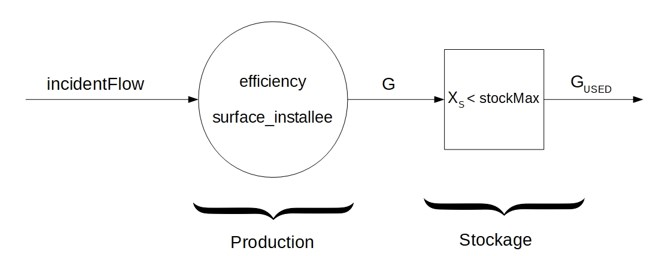
\includegraphics[width=0.75\textwidth]{figures/FeuilleFlux.jpg}
	\caption{text}
	\label{fig:FlowSheet}
\end{figure}

\subsubsection{Flow sheet parameters}

A flow sheet is initially defined by the set of limited parameters listed below (the values are given as an example):

\begin{itemize}
\item \textit{type : flow}

\item \textit{name : solar energy}

\item Incident flow ---  \textit{incidentFlow : 1e10}

\item Conversion efficienc ---  \textit{eff\_init : 0.15}

\item Installed surface ---  \textit{surface\_installee : 1e-9}

\item Usable as energy ---  \textit{isEnergy : True }

\item Maximum storage capacity ---  \textit{stockMax\_init : 50}
\end{itemize}

\subsection{Structure of the physical core}

The physical core is the place where manufactured goods are made. The structure diagram of how this area works is shown in the figure~\ref{fig:kernel}.

\begin{figure}[h]
	\centering 
	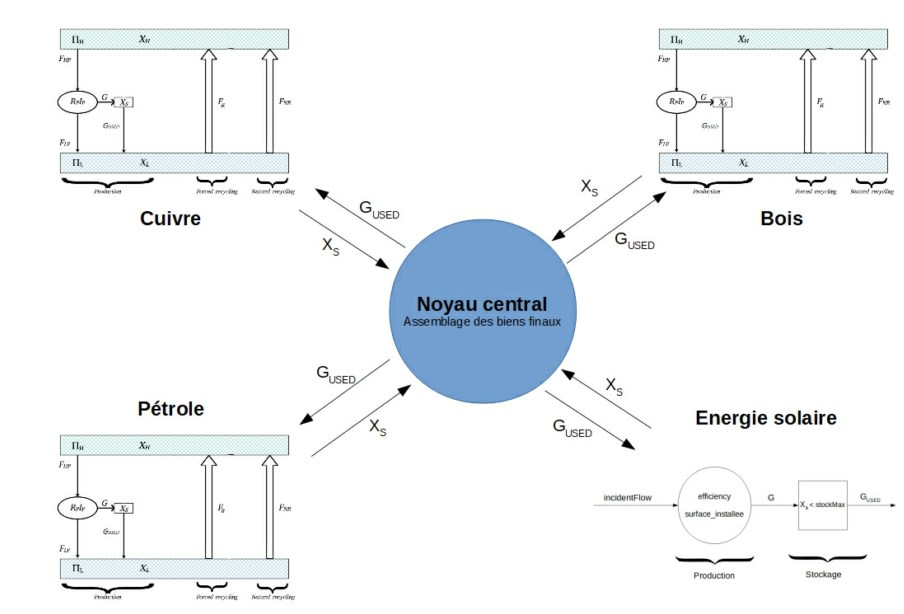
\includegraphics[width=0.75\textwidth]{figures/NoyauCentral.jpg}
	\caption{text}
	\label{fig:kernel}
\end{figure}

The ``recipes'' for the production of manufactured goods are indicated in the sheet \textit{world.txt}. The \textit{main.py} program carries out automatically the realization in respect of these ``recipes''.

\subsection{Structure of the economic zone}

The economic zone is the place where the economic model is coded. To illustrate this point, two examples are given~:

\begin{enumerate}
\item Goodwin

\item Sollow
\end{enumerate}

The advanced user can build his own model following the general structure of an economic structure of an economic sheet (see Appendix~A)







\section{Simulate with \ed}

\subsection{List of files}

You must have in a folder:

\begin{itemize}
	\item the python scripts :
	
	\begin{itemize}
		\item the file \textbf{PhysicalWorld.py}
		
		\item a file describing your economic sphere. In this manual we will use the Goodwin model, described in \textbf{Goodwin.py}.
		
		\item the file \textbf{main.py}
	\end{itemize}
\end{itemize}

\begin{itemize}
	\item as many parameterization files as necessary. At least one resource sheet must be used.
	
	\begin{itemize}
		\item \textbf{world.txt} (required)
		
		\item \textbf{oil.txt} if you have an oil sheet
		
		\item \textbf{copper.txt} if you have a copper sheet
		
	\end{itemize}
\end{itemize}

The file \textbf{main.py} can then be run to launche the simulation. The time step \textit{deltat}, and the temporal extent of the simulation \textit{tmax} can be mofied in \textbf{main.py}.

\subsection{Physical sphere settings}

To modify the physical parameters (cell parameters, and global parameters of the physical sphere), it is necessary to modify the \textbf{*.txt} files.

\subsubsection{Add a cell}

Parameter setting of the new cell:
\begin{enumerate}
	\item to create a stock cell, take the template \textbf{StockCell.txt}, enter the desired parameters, and save under the name of the resource (\textit{e.g.} \textbf{copper.txt})
	
	\item To create a flow cell, do the same with the template \textbf{FlowCell.txt}
	
	\item then, add in \textbf{world.txt} your new cell in the \textit{cells} table.
	
	\item finally, add the column corresponding to recipeMatrix in \textbf{world.txt}
\end{enumerate}

\subsubsection{Retract a cell}

\begin{enumerate}
	\item Delete the cell in the cells table in \textbf{world.txt}
	
	\item Delete the corresponding column from recipeMatrix in \textbf{world.txt}
\end{enumerate}

\subsubsection{Modification of the parameters and initial values of the variables of the physical sphere}

\begin{itemize}
	\item The global parameters and initial values of the global variables of the physical sphere are stored in the \textbf{world.txt} files.
	
	\item The parameters and initial values of the variables of the sheets are stored in the files \textbf{Name-Of-The-Sheet.txt}.
	
	\item Don't forget to save the file \textbf{*.txt} after modifying a value.\footnote{Caution, reading the parameters in the files is {unstable}. You must be careful to respect the spacing, not to add a line break at the end, etc. In particular, the strings in the cell array (e.g. ``~copper.txt~'') are then used to redirect to the file ``~copper.txt~'' for the initialization of the copper sheet. The name of the file containing the parameters of the sheet must therefore be the same string as the one that appears in cell.}
	
	\item The message \texttt{"~world successfully created~"} is printed when the model has been initialized.
\end{itemize}


\subsection{Setting up the economic zone: the Goodwin case}
We show figure~\ref{fig:SetGoodwinParameters} an example of \textit{goodwin.txt} file that set the parameters of the Goodwin economic model.

\begin{figure}[h]
	\centering
	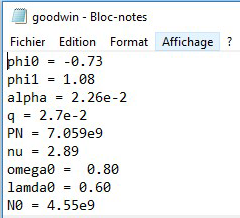
\includegraphics[width=0.3\textwidth]{figures/Goodwin-txt.png}
	\caption{text}
	\label{fig:SetGoodwinParameters}
\end{figure}

\begin{itemize}
	\item $phi0$ and $phi1$ are the parameters of the Philipps curve
	
	\item $alpha$ is the growth rate of labor productivity
	
	\item $q$ is the growth rate of the population
	
	\item $P_{N}$ is the maximum value of the population (the real growth rate of the population $N$ is $q \, (1-N/P_{N}))$)
	
	\item $nu$ is the productivity of capital
	
	\item $omega0$, $lambda0$ and $N_{0}$ are the initial values of the wageshare,
	employment rate and population
\end{itemize}


\section{Elementary case study}

\subsection{Parametrization}

We propose to illustrate the functioning of \ed\ by a case study based on the following:

\begin{itemize}
\item Four resources. Two are material, (copper \textit{Co} and wood \textit{Wo}), and two are energies (oil \textit{Oi} and solar energy \textit{So})

\item  Recipes are build on energy conservation. Three recipes for three different goods are considered~:

	\begin{itemize}
	\item Good 0  can be obtained with 1 unit of copper and 2 units of energy,  
	
	\item Good 1 can be obtained with 1 unit of copper and 2 units of wood and 3 units of energy
	
	\item Good 3 (copper recycling) can be obtained with 1 unit of energy 
	\end{itemize}

\item Target energy mix Mix énergétique cible, is composed of 90\% solar and 10\% oil.
\end{itemize}

\begin{figure}[h]
	\centering
	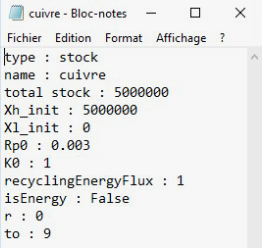
\includegraphics[width=0.3\textwidth]{figures/param_copper.png}
	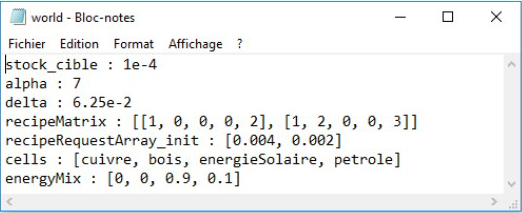
\includegraphics[width=0.65\textwidth]{figures/param_world.png}
	\caption{text}
	\label{fig:parametrization}
\end{figure}

\noindent Screenshots of \textbf{world.txt} and \textbf{copper.txt} parametrization are shown in figure~\ref{fig:parametrization}. In the main file \textbf{main.py}, the following parameters (see figure~\ref{fig:MainParametrization}) must be set~:

\begin{enumerate}
	\item Economic model. Here \textit{Solow}, parameterized by the correspondinf file \textbf{solow.txt} 
	 
	
	\item Time step and the duration of the simulation
\end{enumerate}

\begin{figure}[h]
	\centering
	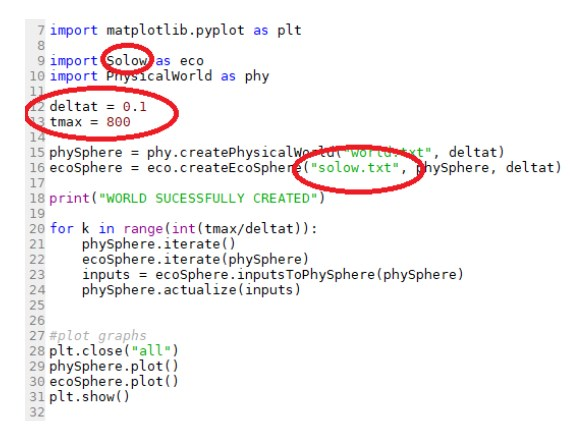
\includegraphics[width=0.5\textwidth]{figures/Parametrisation2.jpg}
	\caption{text}
	\label{fig:MainParametrization}
\end{figure}

%\begin{figure}[h]
%\centering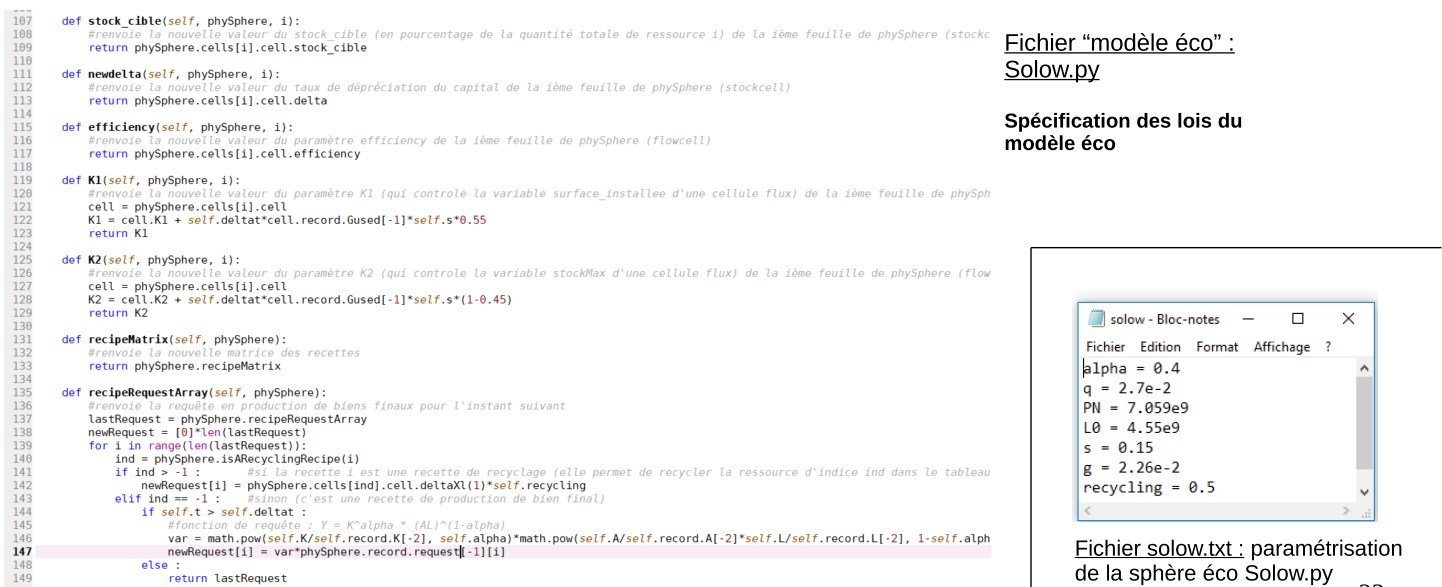
\includegraphics[width=0.95\textwidth]{figures/Parametrisation3.jpg}
%\end{figure}

\subsection{Results}

Running the simulation via the module \textbf{main.py} leads to the results shown in figure~\ref{fig:ResSimulProd} for production and energy. All the information related to each sheet being recorded, it is then possible to follow the specific evolution of their parameters, for example see in figure~\ref{fig:ResSimulOil} for oil.



\begin{figure}[h]
	\centering
	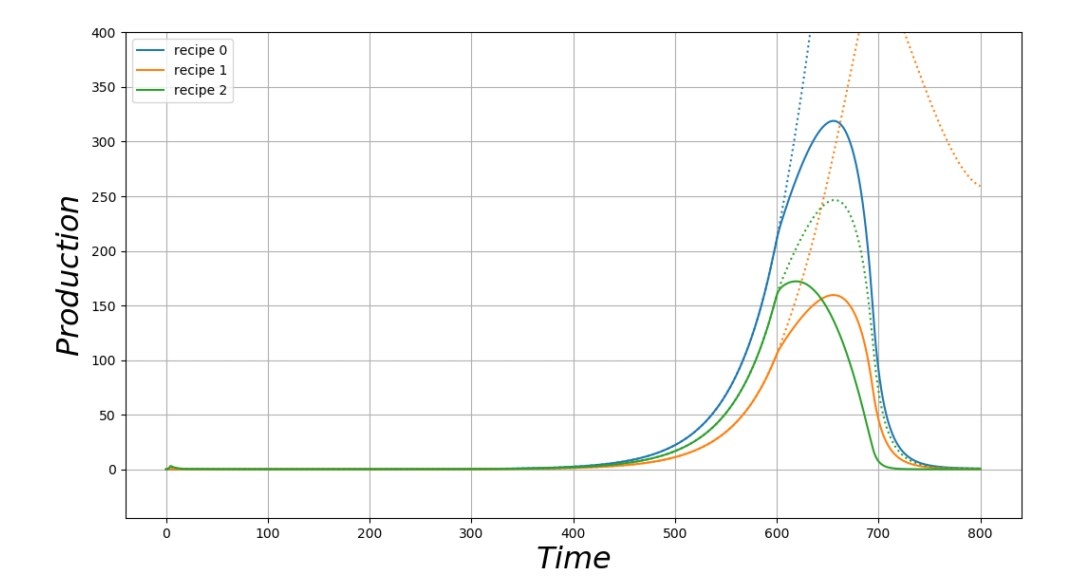
\includegraphics[width=0.45\textwidth]{figures/ResultatSimul.jpg}
	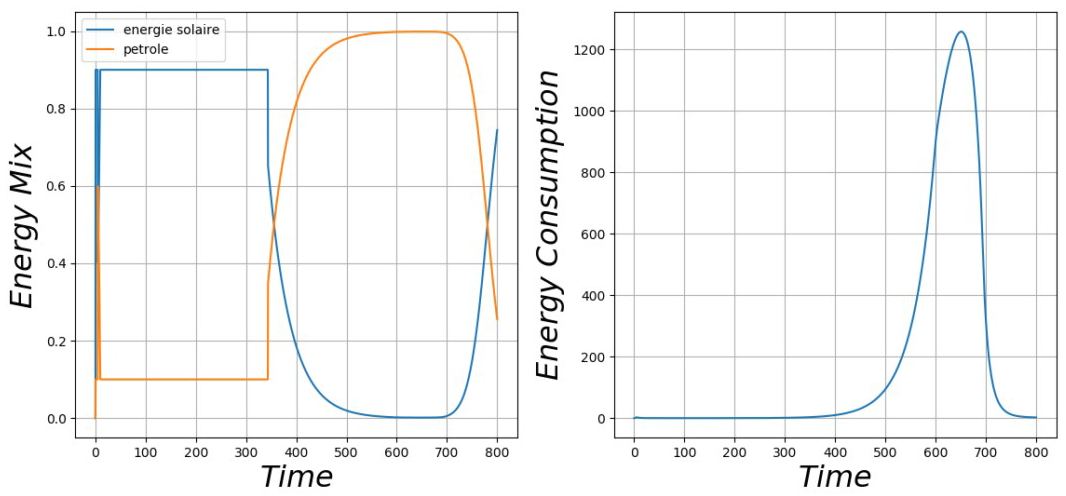
\includegraphics[width=0.51\textwidth]{figures/ResultatSimulE.png}
	\caption{text}
	\label{fig:ResSimulProd}
\end{figure}



\begin{figure}[h]
	\centering
	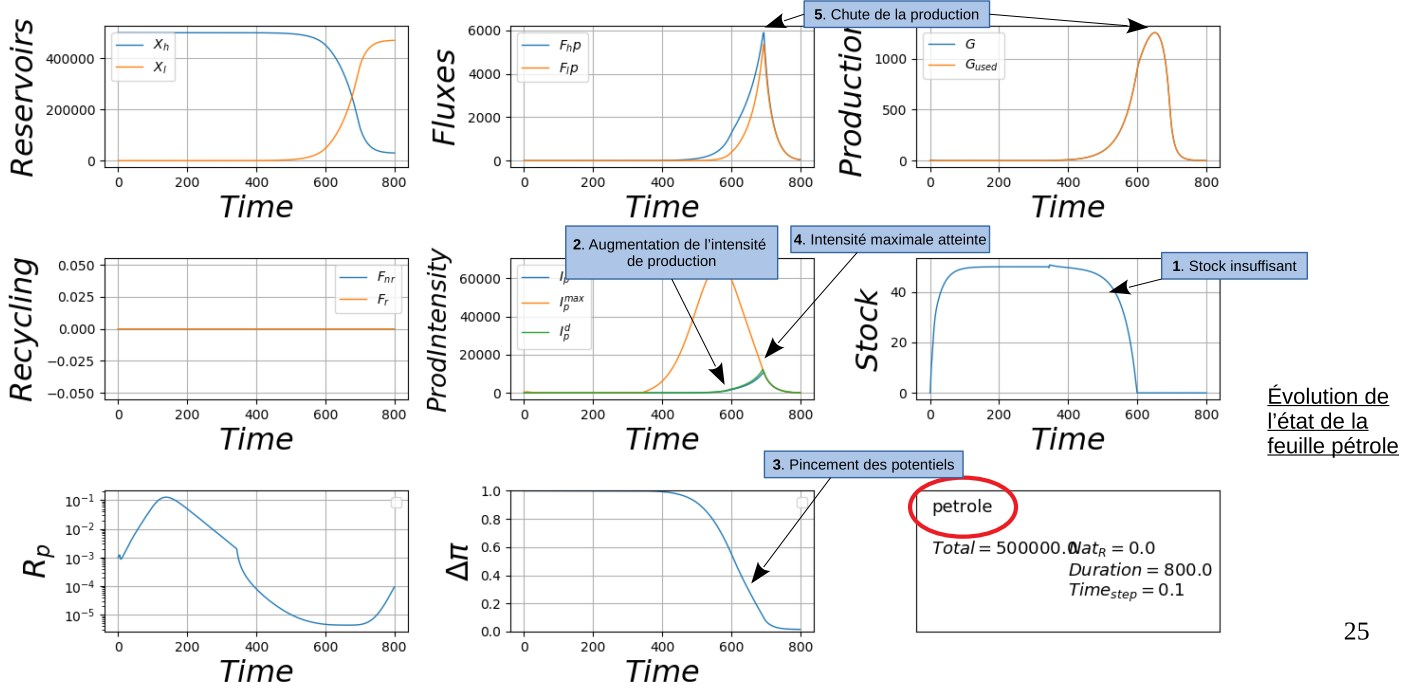
\includegraphics[width=0.9\textwidth]{figures/ResultatSimulPet.jpg}
	\caption{text}
	\label{fig:ResSimulOil}
\end{figure}


\begin{thebibliography}{99}                                                                                               %


\bibitem {Boulinding1966}Boulding, K.E. The economics of the coming spaceship
earth. In Environmental Quality in a Growing Economy.H. Jarrett, Ed.: 3--14.
Johns Hopkins University Press. Baltimore, 1966.

\bibitem {Roegen1971}Georgescu-Roegen, N. The Entropy Law and the Economic
Process. Harvard University Press. Cambridge, MA, 1971.

\bibitem {Sollner1997}Fritz Söllner, A reexamination of the role of
thermodynamics for environmental economics, Ecological Economics, Volume 22,
Issue 3, Pages 175-201, 1997.

\bibitem {Cutler1997}Cutler J Cleveland, Matthias Ruth, When, where, and by
how much do biophysical limits constrain the economic process?: A survey of
Nicholas Georgescu-Roegen's contribution to ecological economics, Ecological
Economics, Volume 22, Issue 3, Pages 203-223, 1997.

\bibitem {Daly1997a}Herman E Daly, Georgescu-Roegen versus Solow/Stiglitz,
Ecological Economics, Volume 22, Issue 3, Pages 261-266, 1997.

\bibitem {Solow1997}Robert M Solow, Georgescu-Roegen versus Solow-Stiglitz,
Ecological Economics, Volume 22, Issue 3, Pages 267-268, 1997.

\bibitem {Stiglitz1997}Joseph E Stiglitz, Georgescu-Roegen versus
Solow/Stiglitz, Ecological Economics, Volume 22, Issue 3, Pages 269-270, 1997.

\bibitem {Daly1997b}Herman E Daly, Reply to Solow/Stiglitz, Ecological
Economics, Volume 22, Issue 3, Pages 271-273, 1997,

\bibitem {Meadows1972}Meadows, D. H., Meadows, D.H., Randers, J\o rgen, et al.
The limits to growth: a report to the club of Rome (1972). 1972.

\bibitem {Glucina2010}Glucina, M. D. and Mayumi, K, Connecting thermodynamics
and economics. Annals of the New York Academy of Sciences, 1185: 11-29. (2010)

\bibitem {Godard1980}Godard O., Baillon J., Céron J., Substitutions et
économie sociale des ressources naturelles, page 15, 1980
\end{thebibliography}


\end{document}